\documentclass[12pt,letterpaper,]{paper}

\NeedsTeXFormat{LaTeX2e} 

\usepackage{etoolbox} % Required for conditional logic and easily changing commands

\newtoggle{unnumberedsections} % Create toggle for a class option
\settoggle{unnumberedsections}{false} % Default value for the class option
\DeclareOption{unnumberedsections}{\settoggle{unnumberedsections}{true}} % Set the class option toggle if the class option was used in the template

% \DeclareOption*{\PassOptionsToClass{\CurrentOption}{article}} % Pass through any extra options specified to the base class
\ProcessOptions\relax % Process class options

% \LoadClass[twocolumn]{article} % Load the base class

%----------------------------------------------------------------------------------------
%	REQUIRED PACKAGES AND MISC CONFIGURATIONS
%----------------------------------------------------------------------------------------
 
\usepackage[bottom, hang]{footmisc} % Force footnotes to the bottom of the page and to the left margin
\setlength{\footnotemargin}{6pt} % Horizontal space between the footnote marker and text

%----------------------------------------------------------------------------------------
%	MARGINS
%----------------------------------------------------------------------------------------

\usepackage[
	top=2.5cm, % Top margin
	bottom=2.5cm, % Bottom margin
	left=2.25cm, % Left margin
	right=2.25cm, % Right margin
	footskip=1cm, % Space from the bottom margin to the baseline of the footer
	headsep=0.75cm, % Space from the top margin to the baseline of the header
	columnsep=20pt, % Space between text columns (in twocolumn mode)
	%showframe % Uncomment to show frames around the margins for debugging purposes
]{geometry}

%----------------------------------------------------------------------------------------
%	FONTS
%----------------------------------------------------------------------------------------

\usepackage[utf8]{inputenc} % Required for inputting international characters
\usepackage[T1]{fontenc} % Output font encoding for international characters

\usepackage[sc]{mathpazo} % Use the Palatino font

\linespread{1.1} % Increase line spacing slightly

\usepackage{microtype} % Slightly tweak font spacing for aesthetics

%----------------------------------------------------------------------------------------
%	HEADERS AND FOOTERS
%----------------------------------------------------------------------------------------

\usepackage{fancyhdr} % Required for customizing headers and footers
\pagestyle{fancy} % Enable custom headers and footers

\renewcommand{\headrulewidth}{0pt} % Top horizontal rule thickness

% \fancyhf{} % Clear default headers/footers

\fancyhead[L]{\small\textit{Choi 2025} }  
% \fancyhead[L]{\small\textit{Choi 2025} % Left-even page header

\fancyfoot[L]{\footnotesize{} }
% \fancyfoot[RO]{\small\textbf{\thepage}} % Right-odd page footer
% \fancyfoot[LO]{\footnotesize\} % Left-odd page footer
% \fancyfoot[LE]{\small\textbf{\thepage}} % Left-even page footer
% \fancyfoot[RE]{\footnotesize\} % Left-even page footer
 
 
%----------------------------------------------------------------------------------------
%	SECTIONS
%----------------------------------------------------------------------------------------

\usepackage{titlesec} % Required for modifying sections

\iftoggle{unnumberedsections}{ % Conditional logic for the unnumbered sections class options
	\setcounter{secnumdepth}{0} % Don't number sections at any level
}{
	\setcounter{secnumdepth}{2} % Number sections down to subsections
}

\titleformat
	{\section} % Section type being modified
	[block] % Section layout type, can be: hang, block, display, runin, leftmargin, rightmargin, drop, wrap, frame
	{\Large\bfseries\centering} % Text formatting of the whole section, i.e. label and title
	{\thesection} % Section label (e.g. number) and its formatting
	{0.5em} % Horizontal space between the section label and title
	{} % Code before the section title
	[] % Code after the section title

%------------------------------------------------

\titleformat
	{\subsection} % Section type being modified
	[block] % Section layout type, can be: hang, block, display, runin, leftmargin, rightmargin, drop, wrap, frame
	{\raggedright\large\bfseries} % Text formatting of the whole section, i.e. label and title
	{\thesubsection} % Section label (e.g. number) and its formatting
	{0.5em} % Horizontal space between the section label and title
	{} % Code before the section title
	[] % Code after the section title

%------------------------------------------------

\titleformat
	{\subsubsection} % Section type being modified
	[runin] % Section layout type, can be: hang, block, display, runin, leftmargin, rightmargin, drop, wrap, frame
	{\bfseries} % Text formatting of the whole section, i.e. label and title
	{} % Section label (e.g. number) and its formatting
	{5pt} % Horizontal space between the section label and title
	{} % Code before the section title
	[] % Code after the section title

\titlespacing*{\subsubsection}{0pt}{0.5\baselineskip}{8pt} % Spacing around section titles, the order is: left, before and after

%----------------------------------------------------------------------------------------
%	TITLE SECTION CUSTOMIZATION
%----------------------------------------------------------------------------------------

\usepackage{titling} % Required for customizing the title section

\setlength{\droptitle}{-4\baselineskip} % Move the title up

\pretitle{\begin{center}\huge\bfseries} % Article title pre-formatting
\posttitle{\end{center}} % Article title post-formatting

\setlength{\thanksmarkwidth}{3pt} % Left margin for the first \thanks line
\setlength{\thanksmargin}{-3pt} % Left margin for the second and onwards \thanks line

\patchcmd{\maketitle}{plain}{empty}{}{} % Set the headers and footers style for the first page to empty

%----------------------------------------------------------------------------------------
%	ABSTRACT CUSTOMIZATION
%----------------------------------------------------------------------------------------

\usepackage{abstract} % Allows abstract customization

\renewcommand{\abstractnamefont}{\normalfont\bfseries\vspace{0.5\baselineskip}} % Set the "Abstract" text to bold
\renewcommand{\abstracttextfont}{\vspace{-0.5\baselineskip}\normalfont\small\itshape} % Set the abstract itself to small italic text
 
%----------------------------------------------------------------------------------------
%	TABLES
%----------------------------------------------------------------------------------------

\usepackage{booktabs} % Required for better horizontal rules in tables

\usepackage{array} % Required for manipulating table columns

\newcolumntype{R}[1]{>{\raggedleft\arraybackslash}p{#1}} % Define a new right-aligned paragraph column type
\newcolumntype{L}[1]{>{\raggedright\arraybackslash}p{#1}} % Define a new left-aligned (no justification) paragraph column type
\newcolumntype{C}[1]{>{\centering\arraybackslash}p{#1}} % Define a new centered paragraph column type

%----------------------------------------------------------------------------------------
%	CAPTIONS
%----------------------------------------------------------------------------------------

\usepackage{caption} % Required for customizing captions

\captionsetup{skip=6pt} % Vertical whitespace between figures/tables and the caption (default is 10pt)
\captionsetup{labelfont={bf,small}, textfont={it,small}} % Define caption font style

%----------------------------------------------------------------------------------------
%	LISTS
%----------------------------------------------------------------------------------------

\usepackage{enumitem} % Required for list customization

\setlist{noitemsep} % Customize spacing around and inside lists

%----------------------------------------------------------------------------------------
%	LINKS
%----------------------------------------------------------------------------------------

\usepackage{hyperref} % Required for links

\hypersetup{
	colorlinks=true, % Whether to color the text of links
	urlcolor=black, % Color for \url and \href links
	linkcolor=black, % Color for \nameref links
	citecolor=black, % Color of reference citations
}

%----------------------------------------------------------------------------------------
%	CUSTOM COMMANDS
%----------------------------------------------------------------------------------------


\usepackage{ifxetex,ifluatex}

\usepackage{lmodern}

\IfFileExists{microtype.sty}{\usepackage{microtype}}{}

%% The amssymb package provides various useful mathematical symbols
\usepackage{amssymb}
%% The amsthm package provides extended theorem environments
%% \usepackage{amsthm}
\usepackage{amsmath}

%% The lineno packages adds line numbers. Start line numbering with
%% \begin{linenumbers}, end it with \end{linenumbers}. Or switch it on
%% for the whole article with \linenumbers after \end{frontmatter}.





\usepackage[authordate, maxcitenames=1, uniquename=mininit, backend=biber, natbib]{biblatex-chicago}
% \usepackage[]{biblatex}
% \usepackage[backend=biber, style=]{biblatex}
\addbibresource{references.bib}


\providecommand{\tightlist}{%
  \setlength{\itemsep}{0pt}\setlength{\parskip}{0pt}}

\setcounter{page}{1} % The page number of the first page, set this to a higher number if the article is to be part of an issue or larger work

 

\setlength{\parindent}{0pt}
\setlength{\parskip}{6pt plus 2pt minus 1pt}
\setlength{\emergencystretch}{3em}  % prevent overfull lines




  
\usepackage{authblk}
 
\author[1 ,$\ast$ ]{Jae S. Choi}

\affil[1]{Bedford Institute of Oceanography, Fisheriess and Oceans
Canada}

\affil[*]{jae.choi@dfo-mpo.gc.ca}
%%------------/AUTHORS--------------


% % Affiliations are output in the \date{} command
% \date{\footnotesize\textsuperscript{\textbf{1}}School of Chemistry, The University of Michigan\\ \textsuperscript{\textbf{2}}Physics Department, The University of Wisconsin\\ \textsuperscript{\textbf{3}}Biological Sciences Department, The University of Minnesota}
\date{\today}

% Full-width abstract
\renewcommand{\maketitlehookd}{%
	\begin{abstract}
		\noindent Snow crab (\emph{Chionoecetes opilio}) are cold-water
stenotherms in the northern hemisphere. As they are long-lived and have
a complex life history, developing an operational model of population
dynamics of snow crab in an environmentally and spatiotemporally
heterogeneous area, the Scotian Shelf of the northwest Atlantic of
Canada. We address these difficulties by focussing upon a better and
more objective parameterization of snow crab growth based upon surveys
of population size structure.
	\end{abstract}
}


\usepackage{graphicx}
\setkeys{Gin}{keepaspectratio}
% Scale images if necessary, so that they will not overflow the page
% margins by default, and it is still possible to overwrite the defaults
% using explicit options in \includegraphics[width, height, ...]{}
%\setkeys{Gin}{width=\maxwidth,height=\maxheight,keepaspectratio}

% Redefine \includegraphics so that, unless explicit options are
% given, the image width will not exceed the width of the page.
% Images get their normal width if they fit onto the page, but
% are scaled down if they would overflow the margins.
\makeatletter
\def\ScaleIfNeeded{%
  \ifdim\Gin@nat@width>\linewidth
    \linewidth
  \else
    \Gin@nat@width
  \fi
}
\makeatother
\let\Oldincludegraphics\includegraphics
{%
 \catcode`\@=11\relax%
 \gdef\includegraphics{\@ifnextchar[{\Oldincludegraphics}{\Oldincludegraphics[width=\ScaleIfNeeded]}}%
}%

 
 

%----------------------------------------------------------------------------------------
%	TITLE SECTION
%----------------------------------------------------------------------------------------

\title{Growth stanzas from kernel mixture models of snow crab size
frequency}


%----------------------------------------------------------------------------------------

\begin{document}

\maketitle % Output the title section


Keywords - snow crab; Bayesian kernel mixture model; Julia; Turing;
growth model; instar


 
  
%% main text
\section{Introduction}\label{introduction}

The overall growth patterns snow crab is reasonably well understood. Due
to short moult cycles of less than a year in the early stages, growth
can be monitored reasonable. However beyond a size range of
approximately XX mm, inter-molt periods can be 1 or more years in
length. Longevity of snow crab can be from 11 (females) to 15 (males)
years. Long term rearing of snow crab is a challenge as living
conditions are generally less than ideal or at least different in
substantial ways from a natural environment, especially for the larger
sized organisms. This can of course create selection biases, such as
stunting due to environmental stress (over-crowding, feeding
irregularities, water quality, etc.).

There also seems to exist inter-individual and regional-variability in
growth patterns due to the interplay environmental (especially bottom
temperatures and resource availablity) and potentially genetic factors
at large geographic scales, depending upon oceanic currents.
Mark-recapture studies can inform such inference for many species,
however, in snow crab, due to the loss of external tags during molts or
difficulty and expense of internal tags, this cannot be used
effectively.

Observations in more natural settings are also possible by scuba or
remote operated vehicle/camera systems. However, such information is
quite costly and resource intensive and also susceptible to selection
bias in that recaptured or surviving animals tend to be those in better
physiological condition than average and so can result in expectations
of overly optimistic growth patterns. When routine sampling occurs, a
more cost-effective way to establish or corroborate these growth
patterns is to decompose observed size frequency distributions. Though
there is also inherent size-selection biases in such data due to
size-related behavior (habitat preferences) and capture efficiency (net
size, speed, depth) that changes with different size and stages, it is
still possible to extract some meaningful information of size modes from
such data and infer growth patterns.

Given some set of observations of size frequency, subjective ``best
guesses'' (classification by ``eye'') and implicit reasoning can be used
to establish and classify these growth modes. When groups are distinct,
this is reasonable. However, observations of size frequencies often
demonstrate a mixture of distributions that are heavily overlapping.
Even the most state-of-the-art computational algorithms cannot fit such
distributions easily. One of the leading more objective approaches to
estimate classification using point estimates of latent parameters
became available with the development of the Expectation-Maximization
(EM) algorithm operating in an Maximum Likelihood framework (Dempster et
al 1977; see also the closely related Kalman Filter (Roweis and
Ghahramani 1999)) and for distributions in Bayesian frameworks with
Variational Inference (Nguyen 2023) and general latent Bayesian
Inference. Here we use the latter method, more specifically,
\textbf{Kernel Mixture Model (KMM)}, using population census-based data
to identifying growth stanzas using snow crab data derived from the
Maritimes Region of Atlantic Canada.

\section{Methods}\label{methods}

The use of a mixture of distributions has a long history. Pearson (1894)
where it was used to identify/classify species of crabs. Holmes (1892)
also studied mixture models of wealth disparity. Most numerical methods
assigning or classifying data into a cluster or group generally requires
the number of such groups to be specified apriori. The excepton being,
Infinite Mxture Models (Ghahramani 2011). Fortunately, we have a
reasonable understanding of the number of approximate modes of instar
carapace widths from visual analysis of size-frequency distributions.
This process can be automated by

The finite form of the problem is well known and understood.
Implementation is usually with Maximum likelihood using an
Expectation-Maximization algorithm (EM; Dempster, Laird, \& Rubin,
1977). The solutions to such problems are dependent upon the number of
modes chosen, or often the location of the modes, apriori. Many tools
exist for estimation:

\begin{itemize}
\item
  https://cran.r-project.org/web/packages/mixtools/vignettes/mixtools.pdf
\item
  https://cran.r-project.org/web/packages/flexmix/vignettes/bootstrapping.pdf
\item
  https://statmath.wu.ac.at/\textasciitilde gruen/BayesMix/bayesmix-intro.pdf
\end{itemize}

must specify constant node using mcmc Jags

\url{https://cran.r-project.org/web/packages/mclust/vignettes/mclust.html}

problems

\url{https://arxiv.org/pdf/2007.04470}

\url{https://dr.lib.iastate.edu/server/api/core/bitstreams/333bb46d-c759-4202-8f41-0e921271de53/content}

good reviews \url{https://snunnari.github.io/SBE/mclachlan.pdf}

\url{https://en.wikipedia.org/wiki/Mixture_model?wprov=sfti1}

\url{https://www.sciencedirect.com/topics/medicine-and-dentistry/mixture-model}

We can cluster the data using a Bayesian mixture model. The aim of this
task is to infer a a latent grouping (hidden structure) from unlabelled
data.

Unidimensional Kernel Mixture model with K pre-specified components that
cover the space

\(\\alpha\) = concentration parameter of 1 (or k, the dimension of the
Dirichlet distribution, by the definition used in the topic modelling
literature) results in all sets of probabilities being equally likely,
i.e., in this case the Dirichlet distribution of dimension k is
equivalent to a uniform distribution over a k-1-dimensional simplex.
This is not the same as what happens when the concentration parameter
tends towards infinity. In the former case, all resulting distributions
are equally likely (the distribution over distributions is uniform). In
the latter case, only near-uniform distributions are likely (the
distribution over distributions is highly peaked around the uniform
distribution).

label=``observation (i)'', ylabel=``cluster (k)'', legend=false, ) end

https://turing.ml/dev/tutorials/01-gaussian-mixture-model/

\section{Finite mixtures model}\label{finite-mixtures-model}

\url{https://turinglang.org/stable/tutorials/01-gaussian-mixture-model/}

\url{https://mc-stan.org/users/documentation/case-studies/identifying_mixture_models.html}

we want to infer the mixture weights, the parameters
\textbackslash mu\_i and the assignment of each datum to a cluster i

standard normal distributions as priors for \textbackslash mu and a
Dirichlet distribution with parameters \textbackslash alpha\_i as prior
for w

\$\$ \textbackslash begin\{aligned\} \textbackslash mu\_k
\&\textbackslash sim \textbackslash mathcal\{N\}(0, 1)
\textbackslash qquad (k = 1,\textbackslash ldots,K) \textbackslash{} w
\&\textbackslash sim
\textbackslash operatorname\{Dirichlet\}(\textbackslash alpha\_1,
\textbackslash ldots, \textbackslash alpha\_K)
\textbackslash end\{aligned\}

\{\} \textbackslash{} \{\} \textbackslash{}

z\_i \textbackslash sim \textbackslash operatorname\{Categorical\}(w)
\textbackslash qquad (i = 1,\textbackslash ldots,N), \textbackslash{}

\{\} \textbackslash{} x\_i \textbackslash sim
\textbackslash mathcal\{N\}({[}\textbackslash mu\_\{z\_i\},
\textbackslash mu\_\{z\_i\}{]}\^{}\textbackslash mathsf\{T\}, I)
\textbackslash qquad (i=1,\textbackslash ldots,N). \$\$

From simple kernel density representations of size frequency at small
area unit scale, determine the magnitudes of modes. This is done as
there may be regional and time-dependent changes in modal sizes
(year-classes). Sex and maturity status are determined from observation
and infered from size-shape changes (carapace width to chela height
males or abdominal flap width for females). Inference of modal sizes for
each sex-maturity group are determined in order to develop a growth
model.

Kernel density estimates of specific components: sex, maturity, year,
time of year (season in quarters), region and set (sid).

First we construct kernel density estimates using a bandwidth of 0.025
units on a logarithmic scale. This corresponds to about 4 dx (mm), where
dx is the increment width of discretization.

These results are normalized by swept area to provide a density per unit
area (1 km\(^{-2}\)).

\section{Results and Discussions}\label{results-and-discussions}

\begin{verbatim}
            Coef.  Std. Error      t  Pr(>|t|)  Lower 95%  Upper 95%
\end{verbatim}

(Intercept) 1.05187 0.0430406 24.44 \textless1e-04 0.932365 1.17136
instar 0.321978 0.00640426 50.28 \textless1e-06 0.304196 0.339759

(Intercept) 1.49157 0.216241 6.90 0.0917 -1.25602 4.23917 instar
0.268652 0.0221858 12.11 0.0525 -0.0132459 0.550549

(Intercept) 1.10376 0.0259636 42.51 \textless1e-08 1.04237 1.16515
instar 0.308079 0.00308857 99.75 \textless1e-11 0.300775 0.315382

(Intercept) 0.335281 0.114697 2.92 0.2098 -1.12208 1.79264 instar
0.363371 0.00953601 38.11 0.0167 0.242204 0.484537

\begin{figure}
\centering
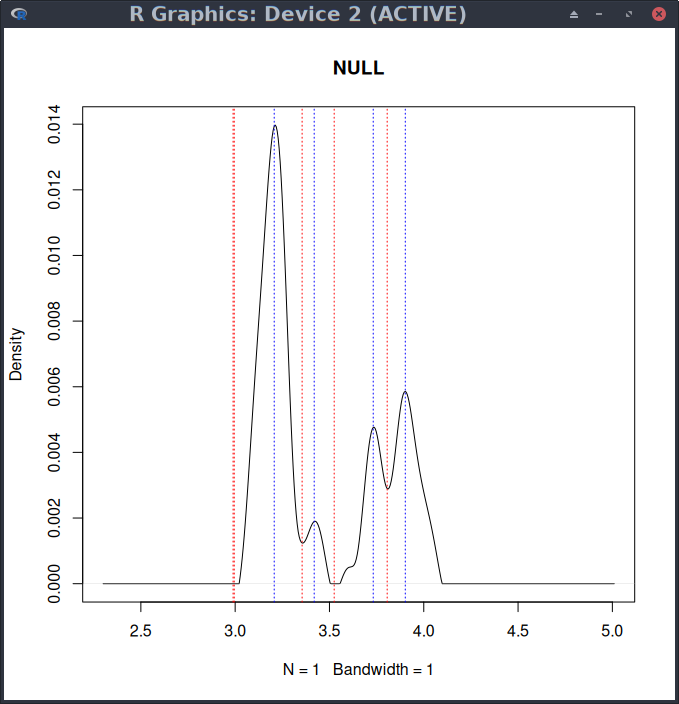
\includegraphics{../../outputs/example_modal_classification_2.png}
\caption{image}
\end{figure}

\begin{figure}
\centering
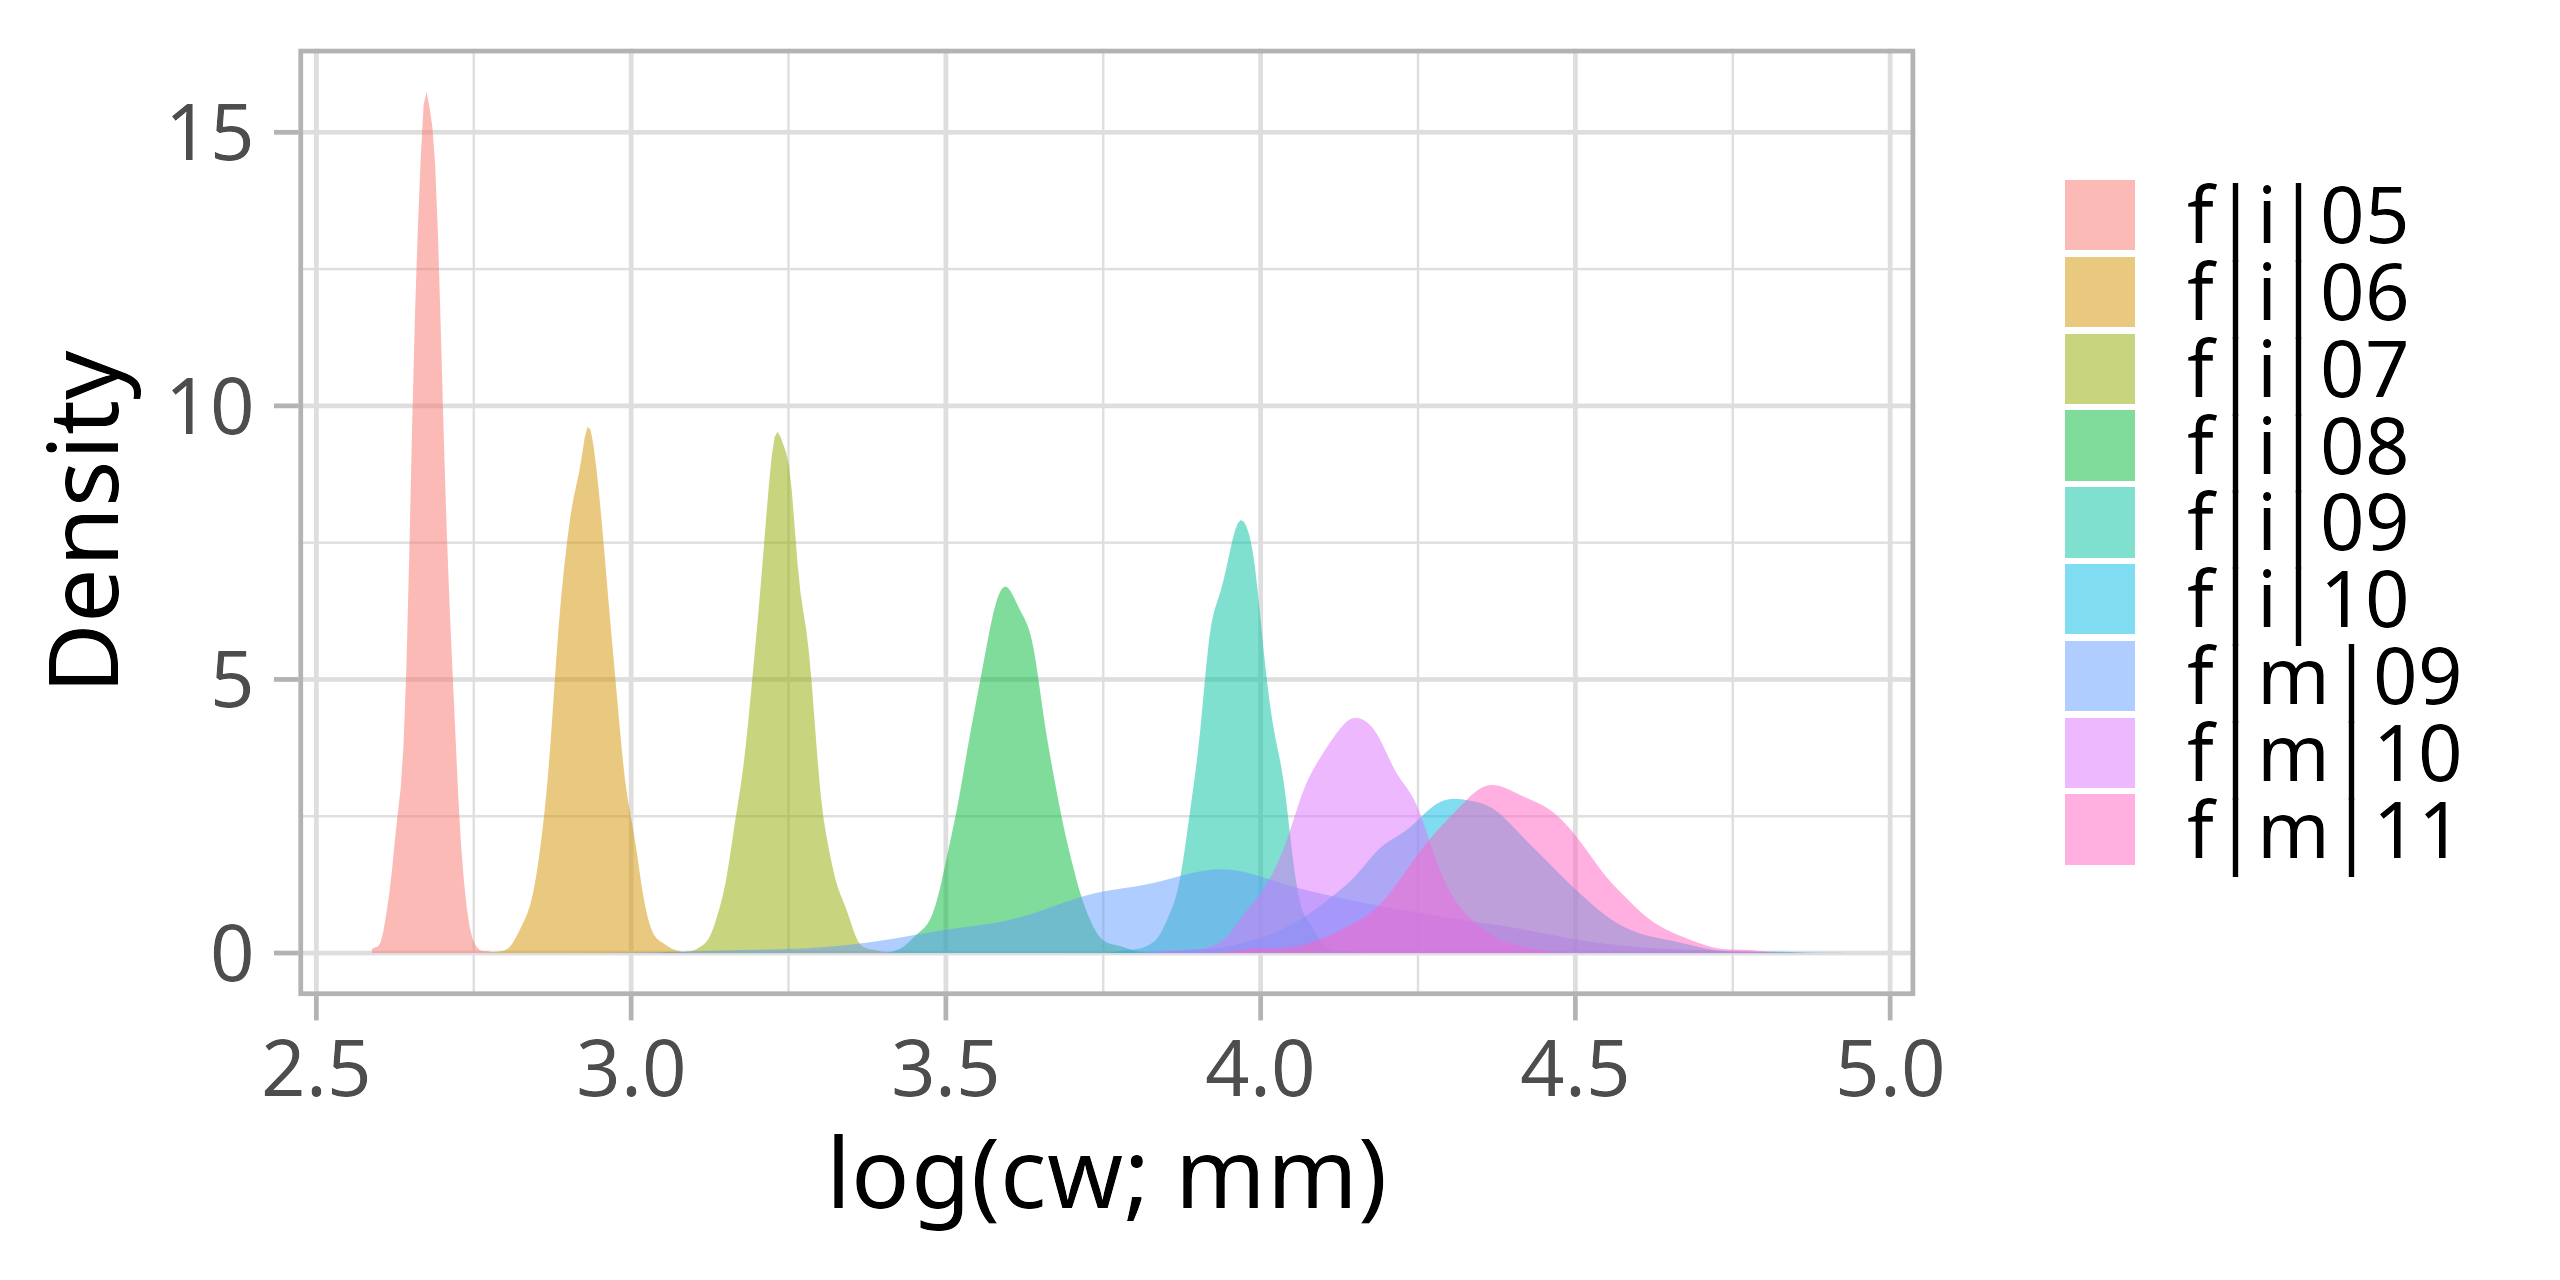
\includegraphics{../../outputs/modelled/figures/density_2020_1_f_imodes.png}
\caption{image}
\end{figure}

\begin{figure}
\centering
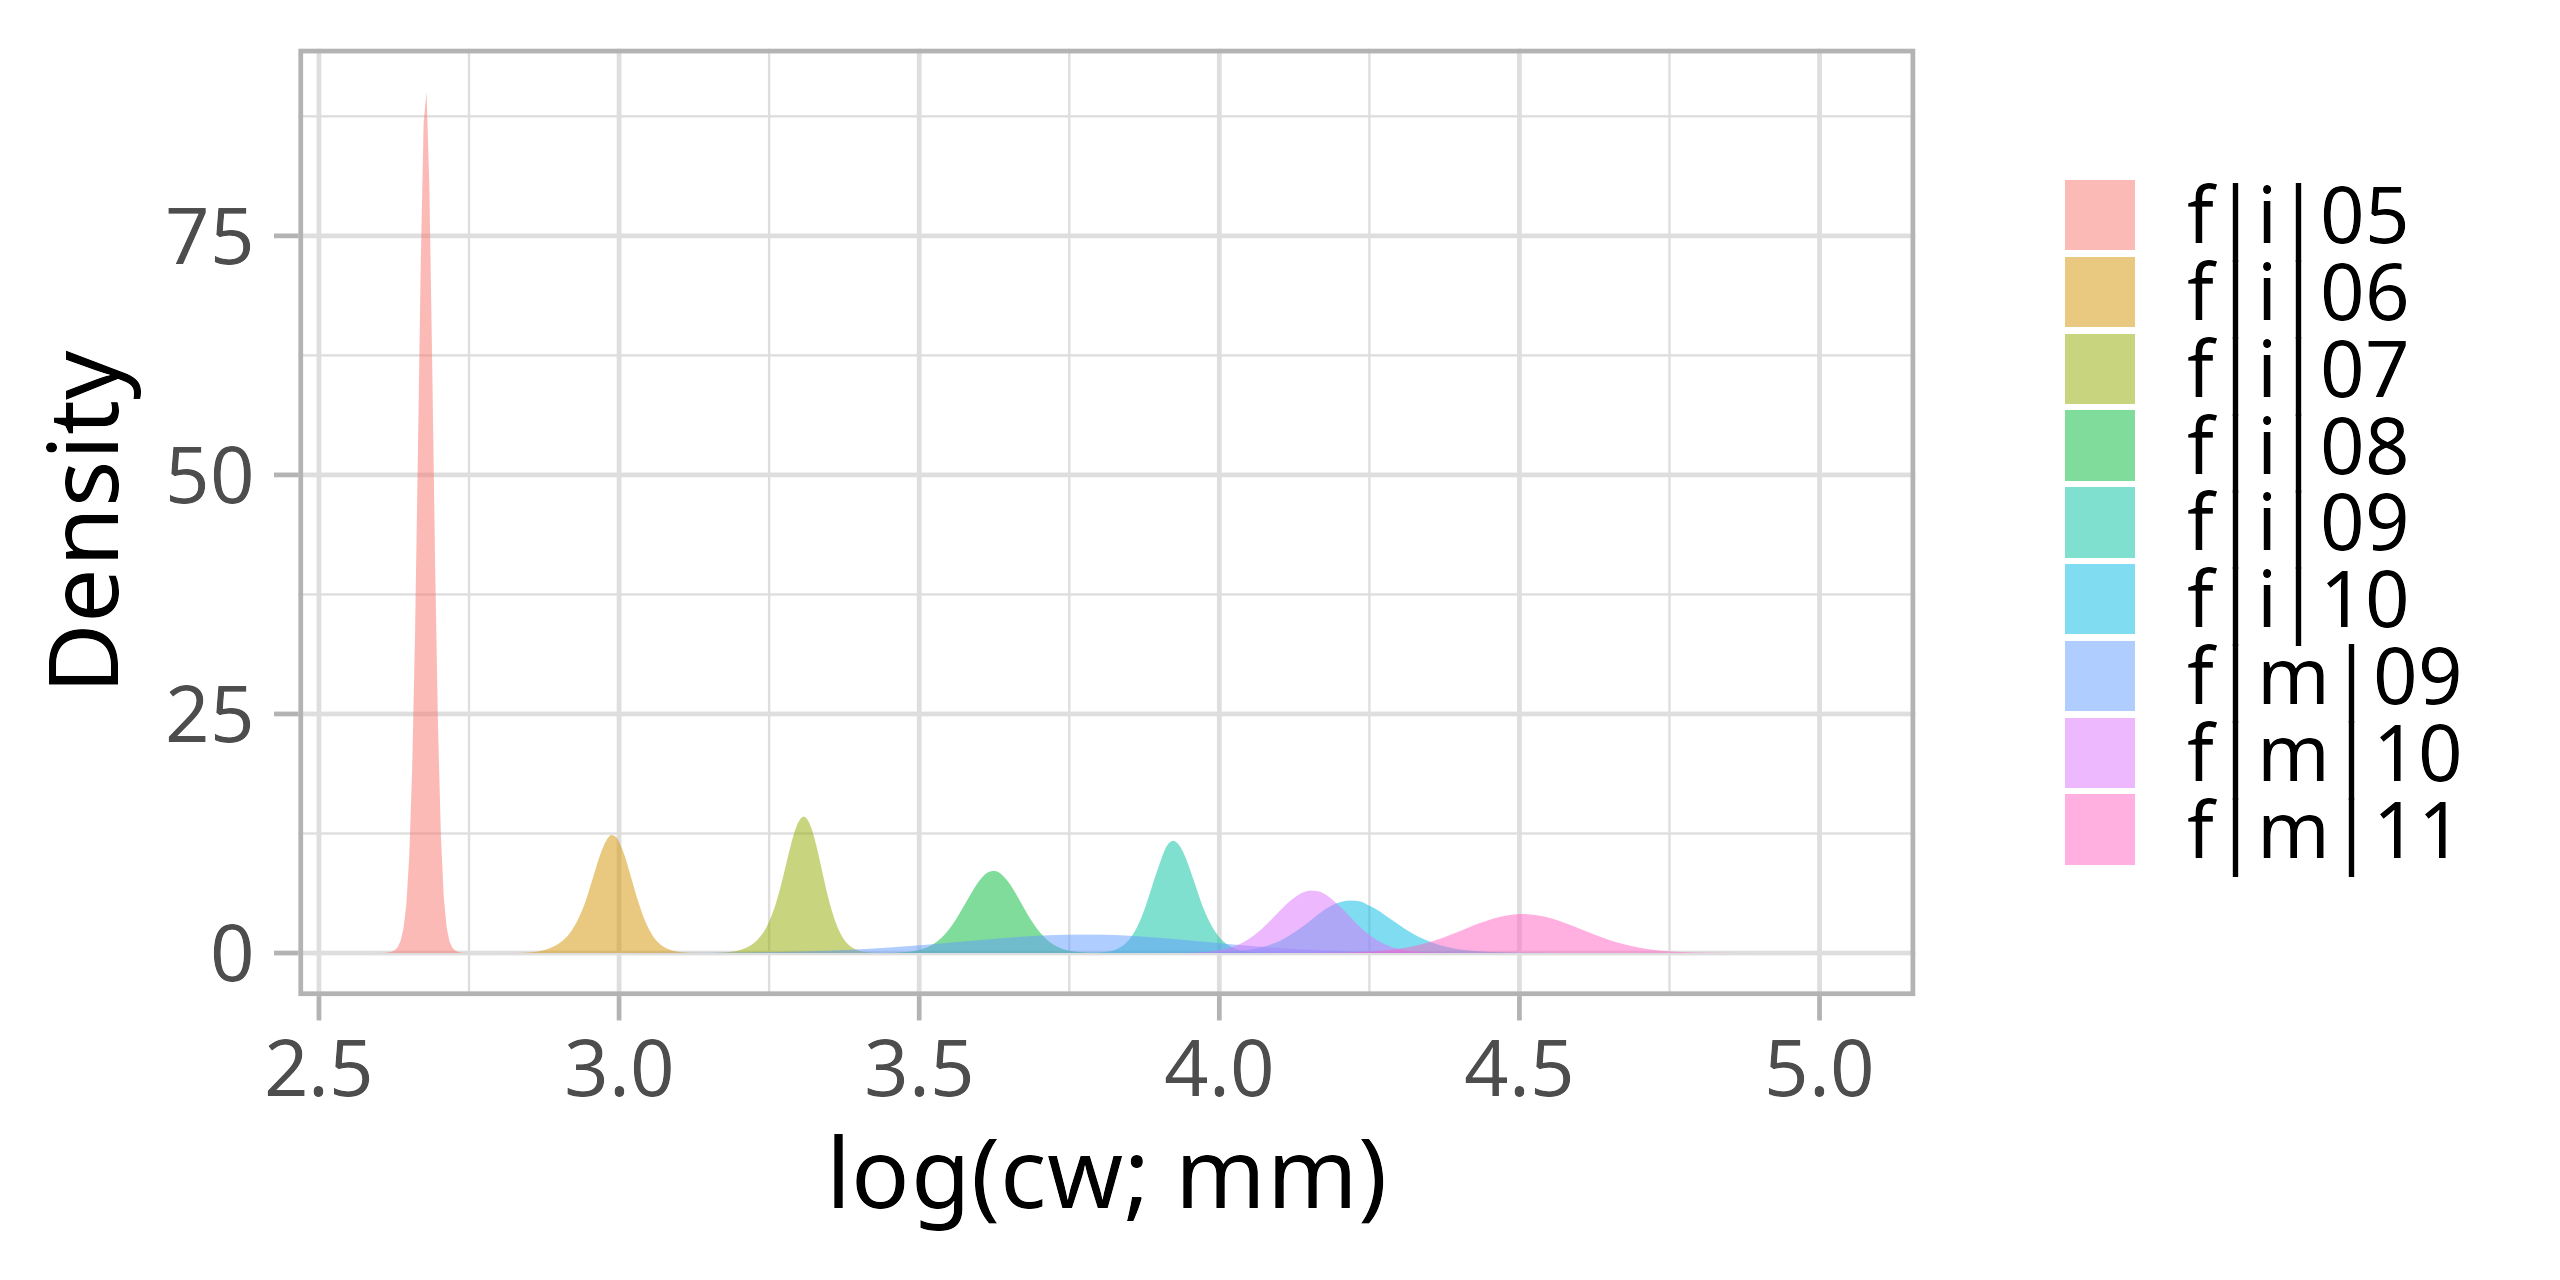
\includegraphics{../../outputs/modelled/figures/density_2020_f_imodes.png}
\caption{image}
\end{figure}

\begin{figure}
\centering
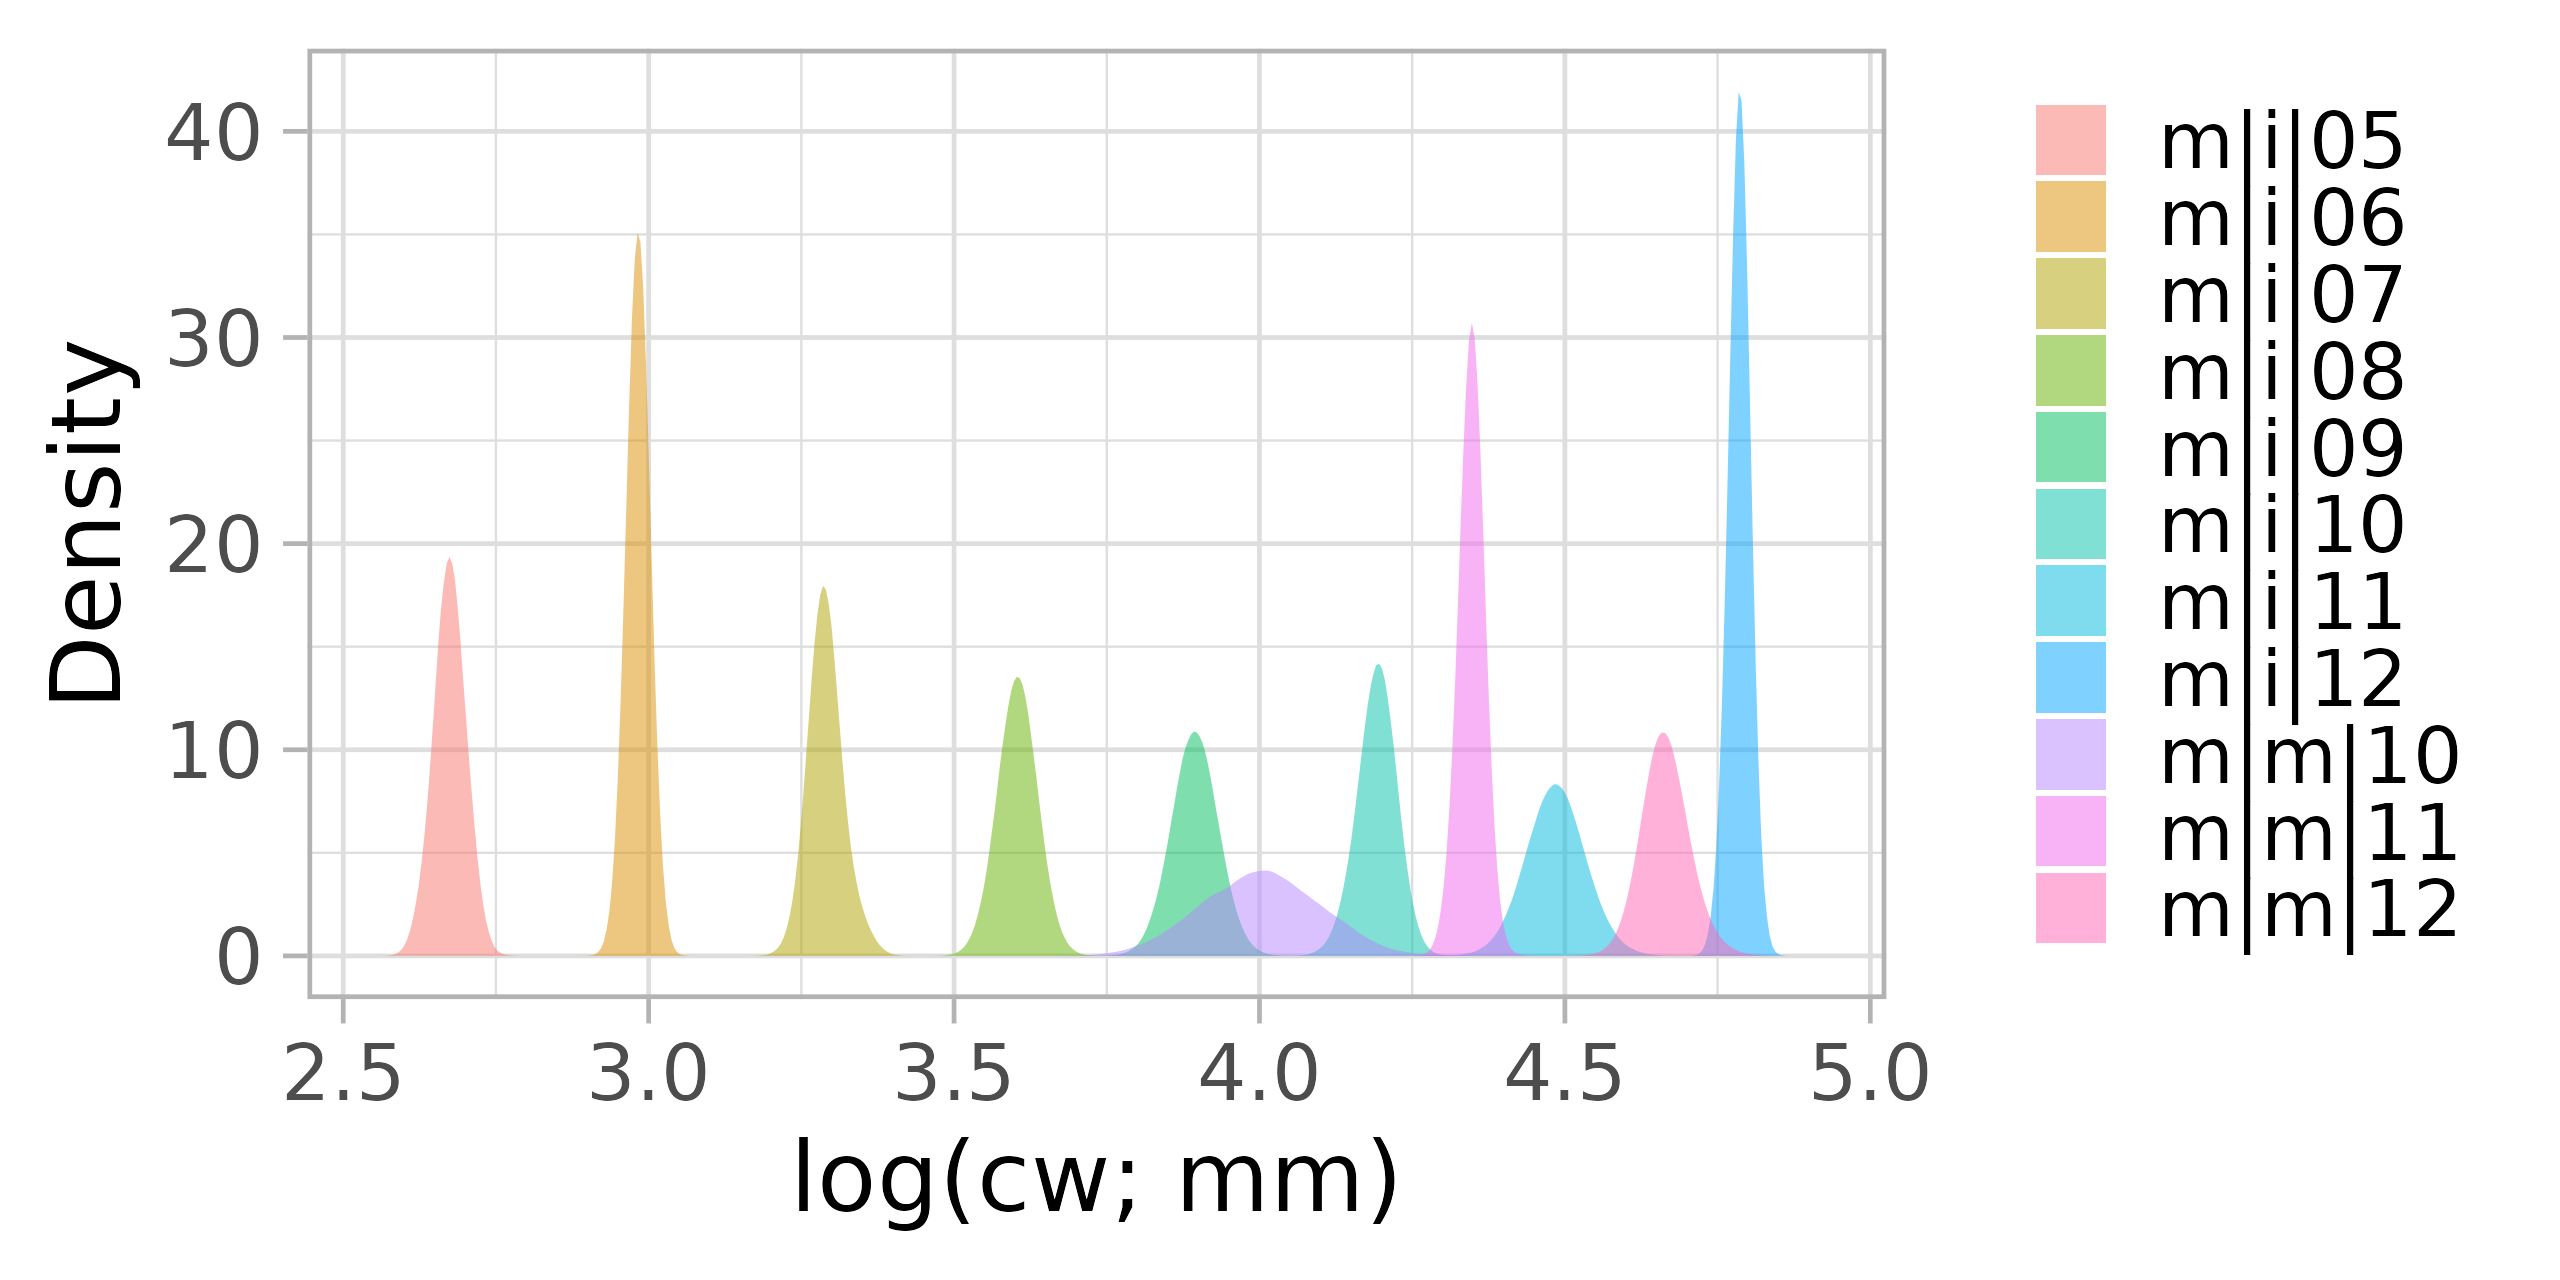
\includegraphics{../../outputs/modelled/figures/density_2020_m_imodes.png}
\caption{image}
\end{figure}

\begin{figure}
\centering
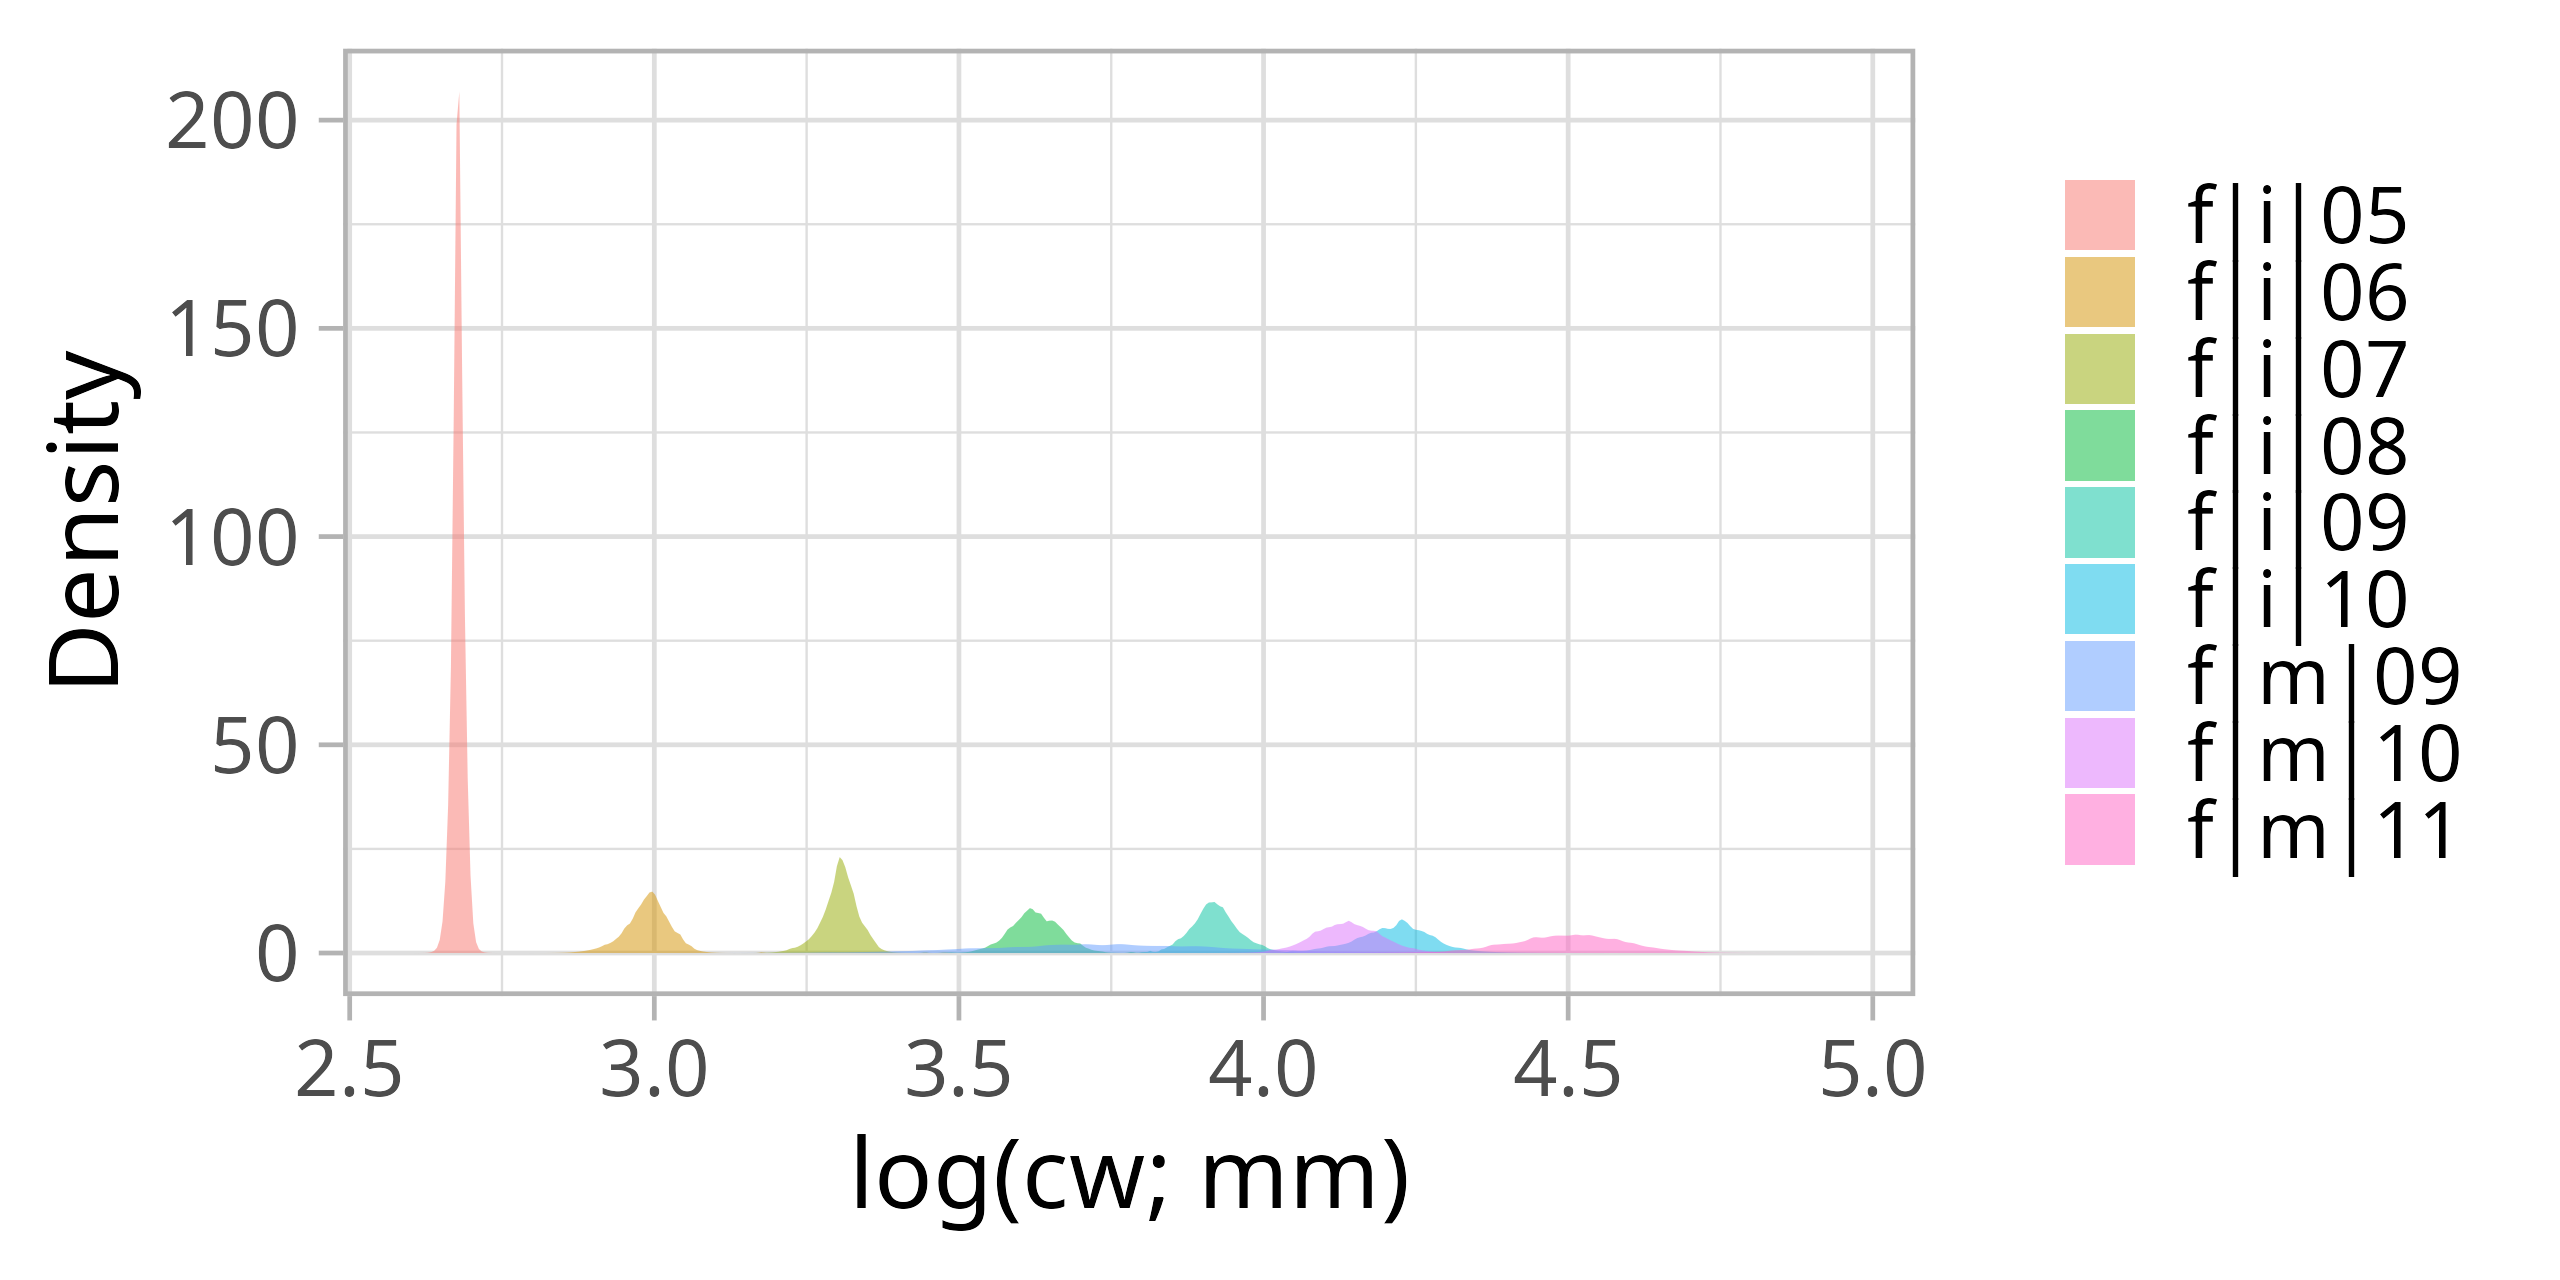
\includegraphics{../../outputs/modelled/figures/density_2021_f_imodes.png}
\caption{image}
\end{figure}

\begin{figure}
\centering
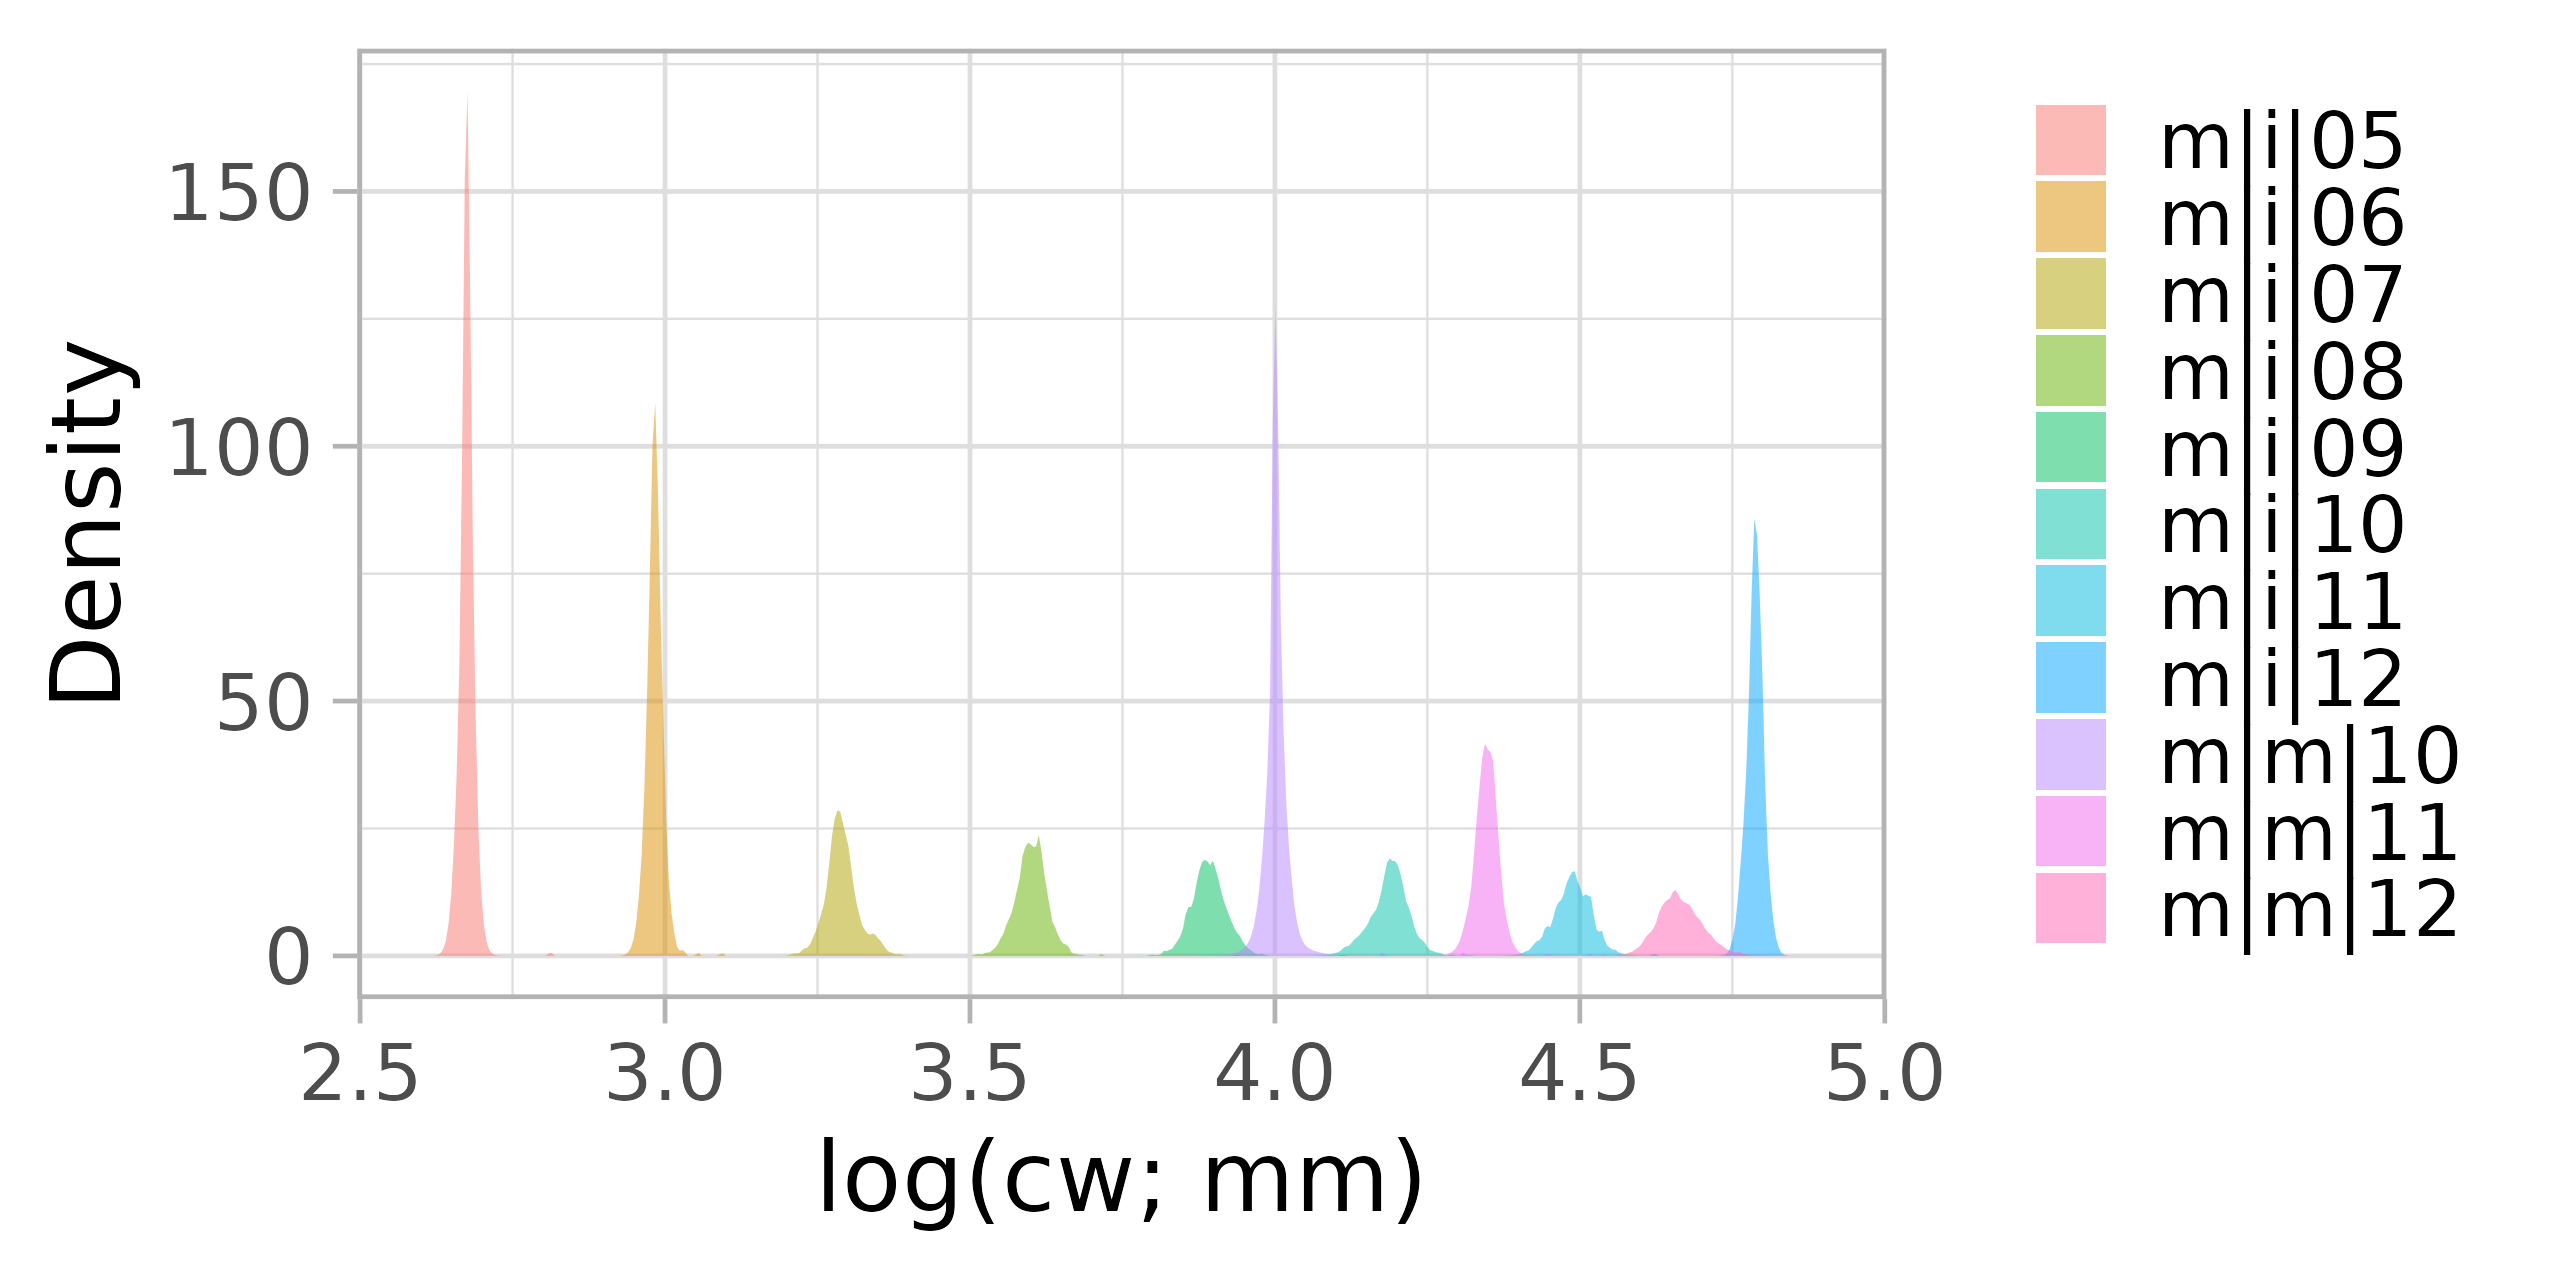
\includegraphics{../../outputs/modelled/figures/density_2021_m_imodes.png}
\caption{image}
\end{figure}

\begin{figure}
\centering
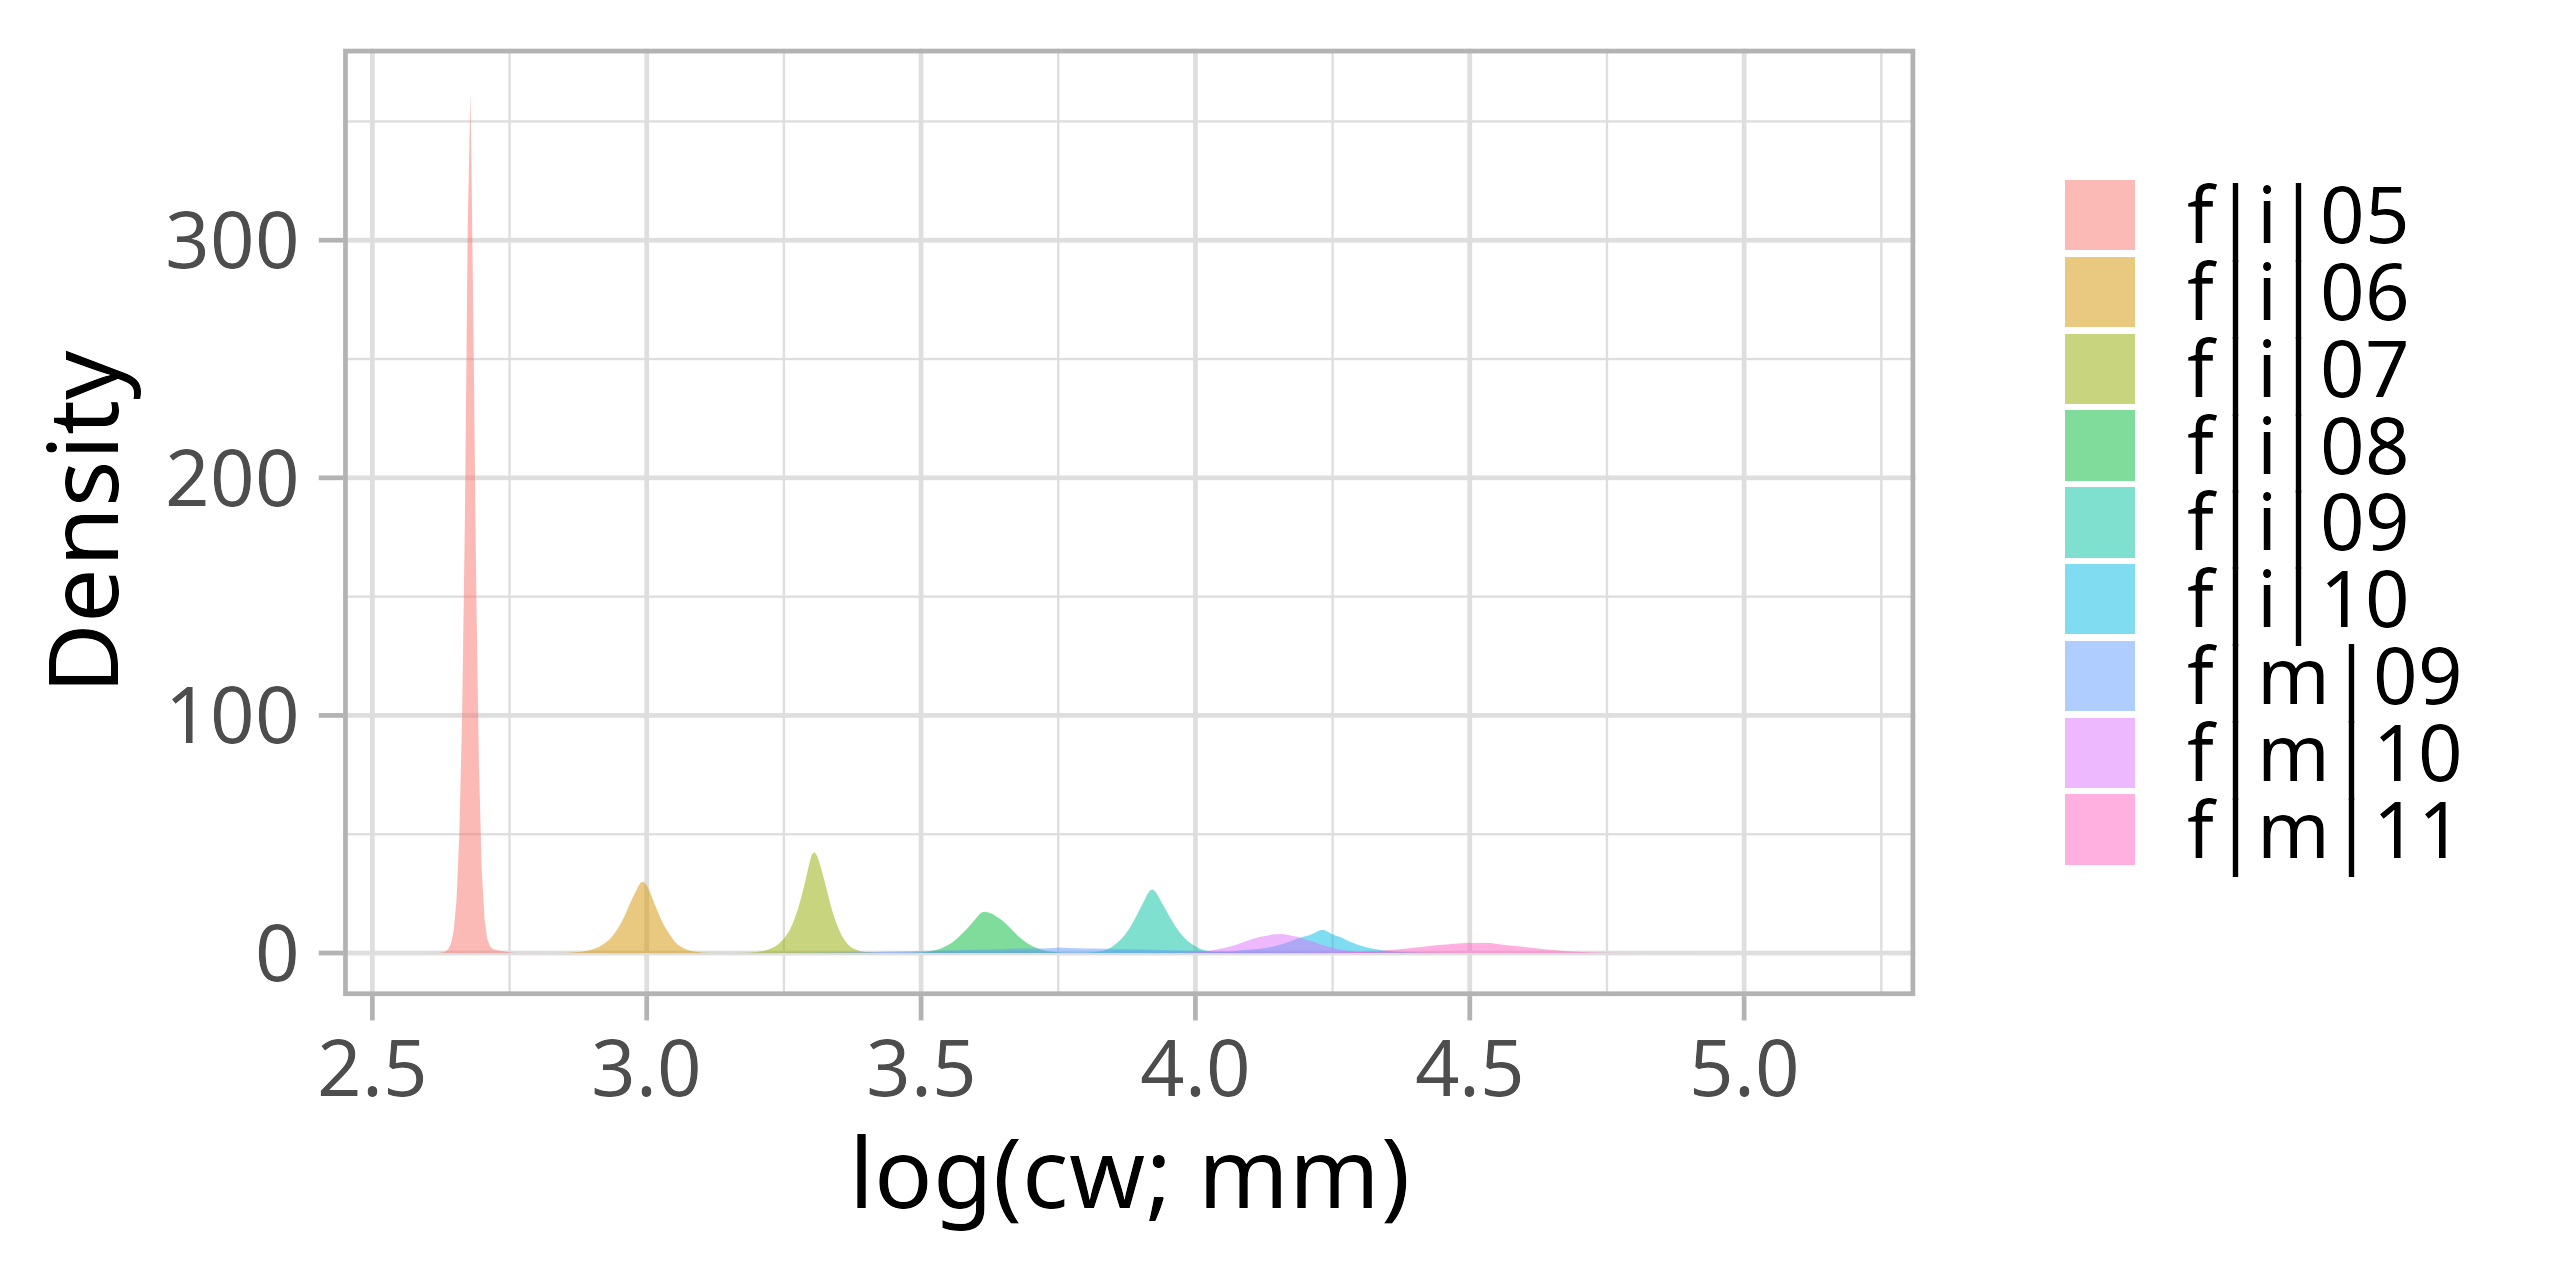
\includegraphics{../../outputs/modelled/figures/density_f_imodes.png}
\caption{image}
\end{figure}

\begin{figure}
\centering
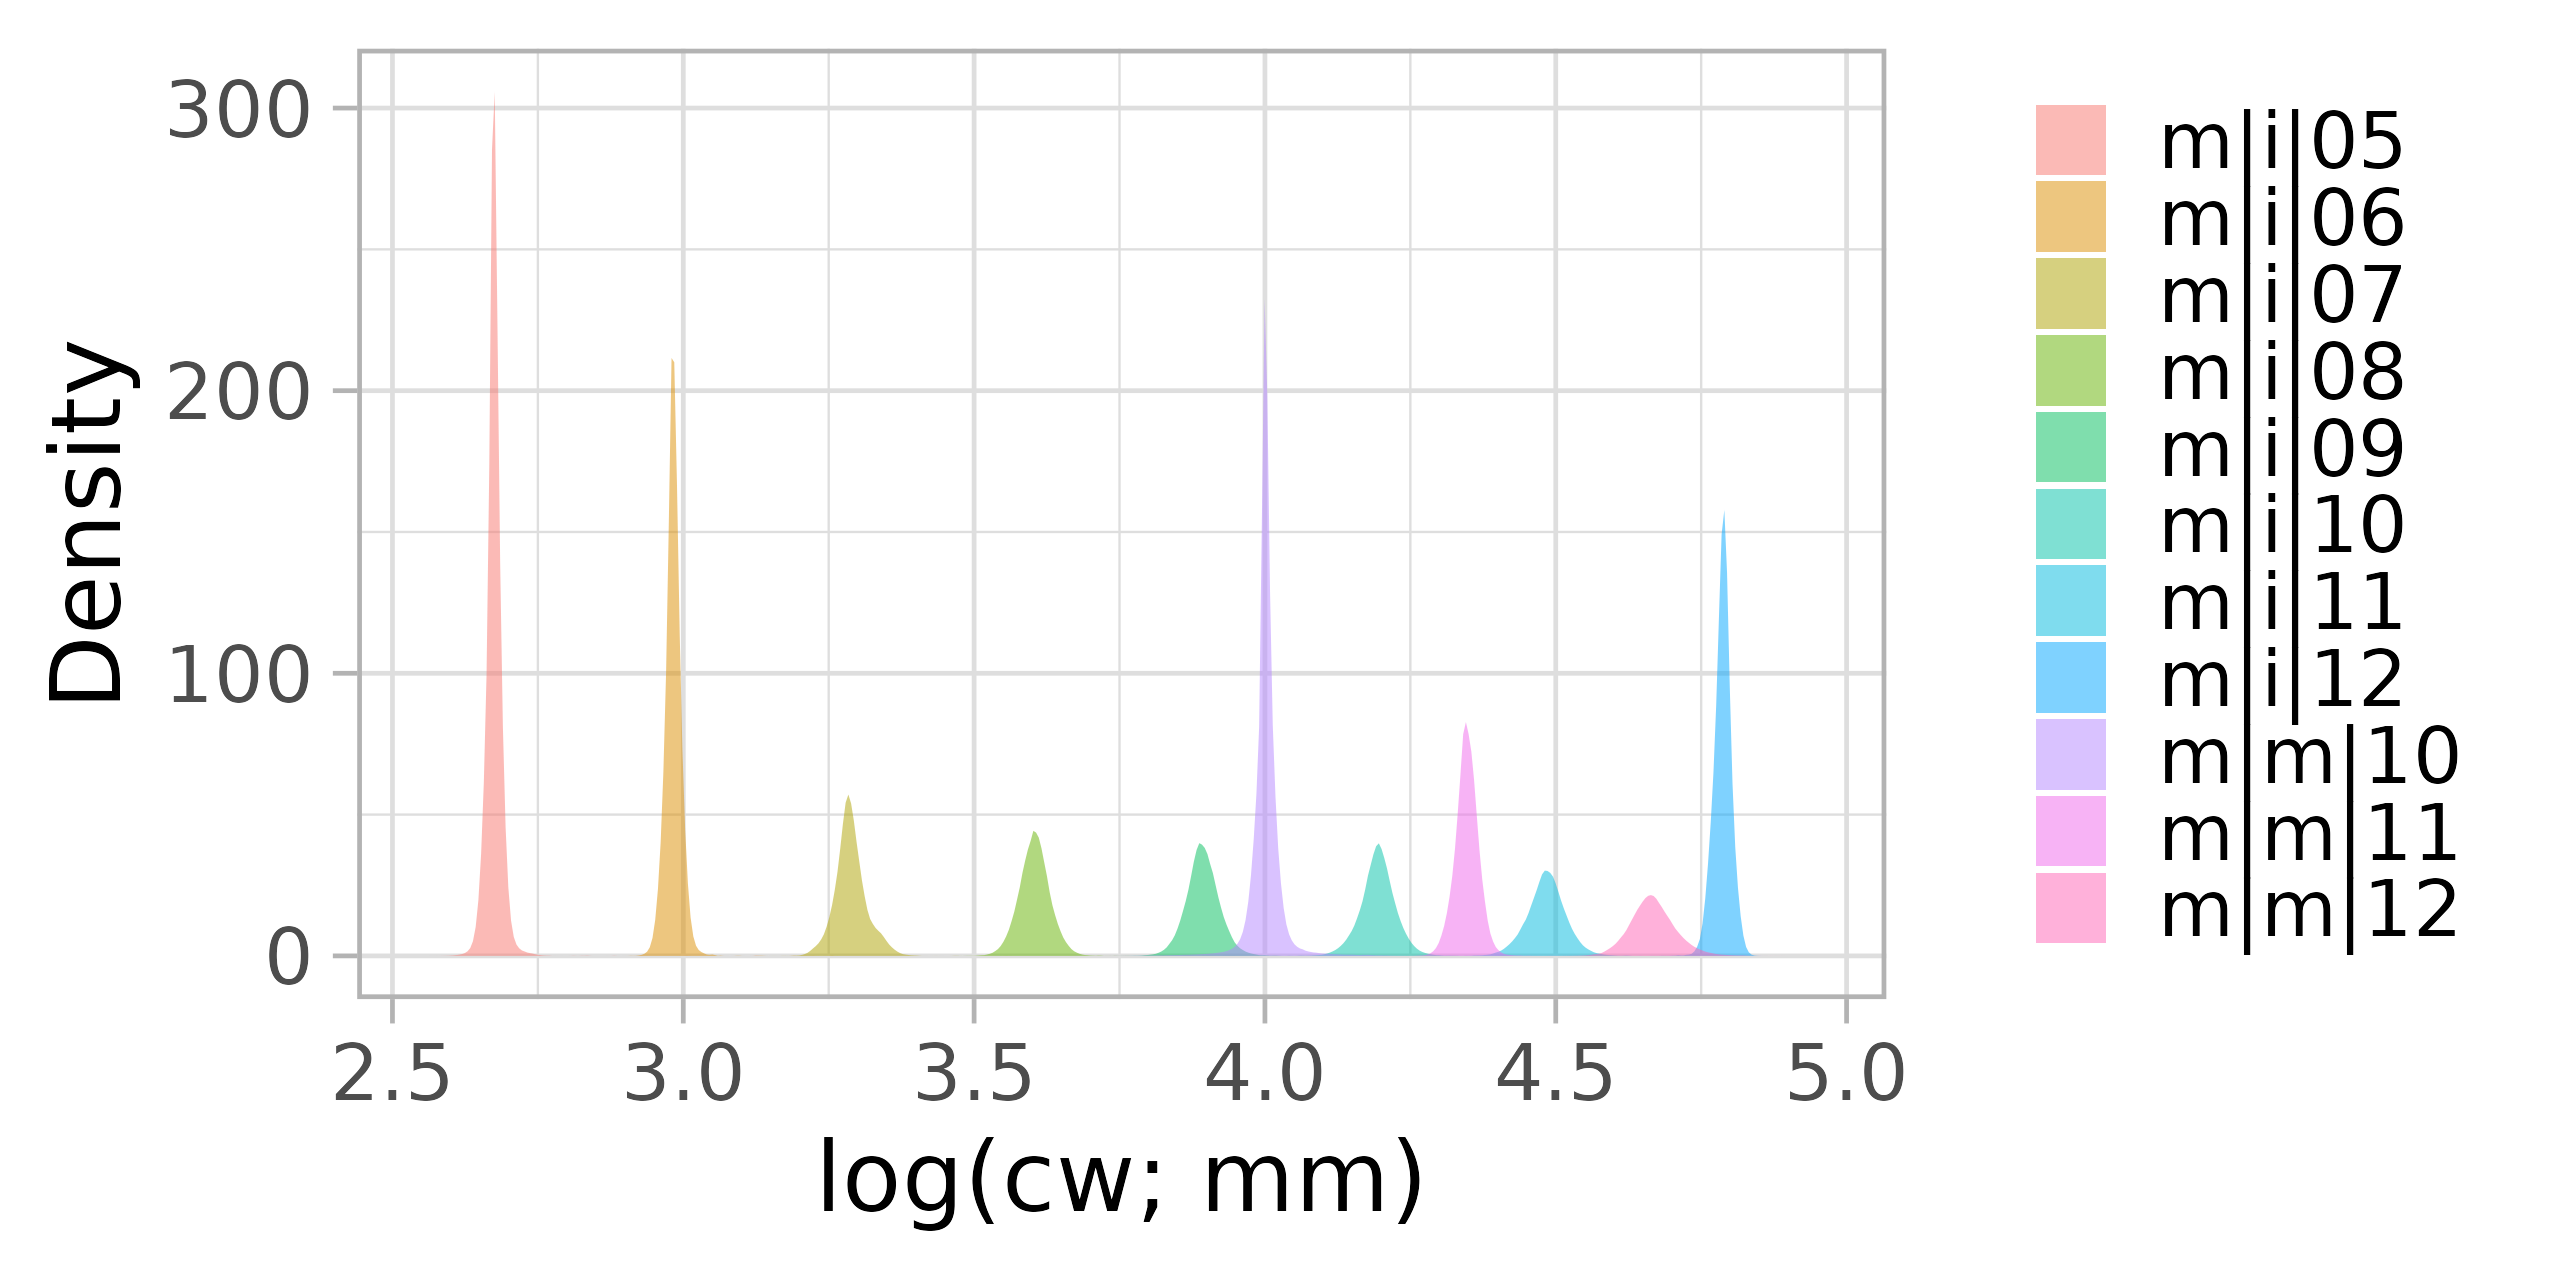
\includegraphics{../../outputs/modelled/figures/density_m_imodes.png}
\caption{image}
\end{figure}

\begin{figure}
\centering
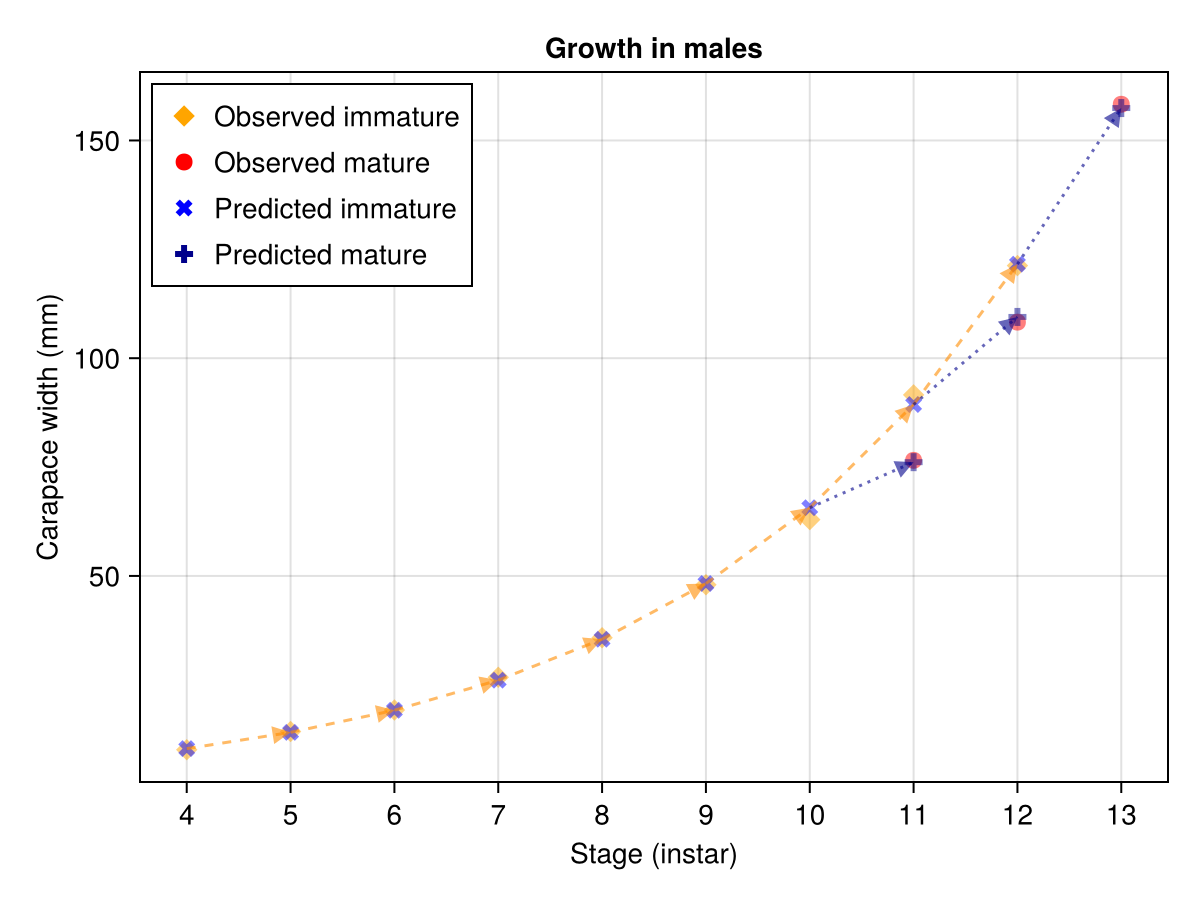
\includegraphics{../../outputs/plot_growth_male.png}
\caption{image}
\end{figure}

\begin{figure}
\centering
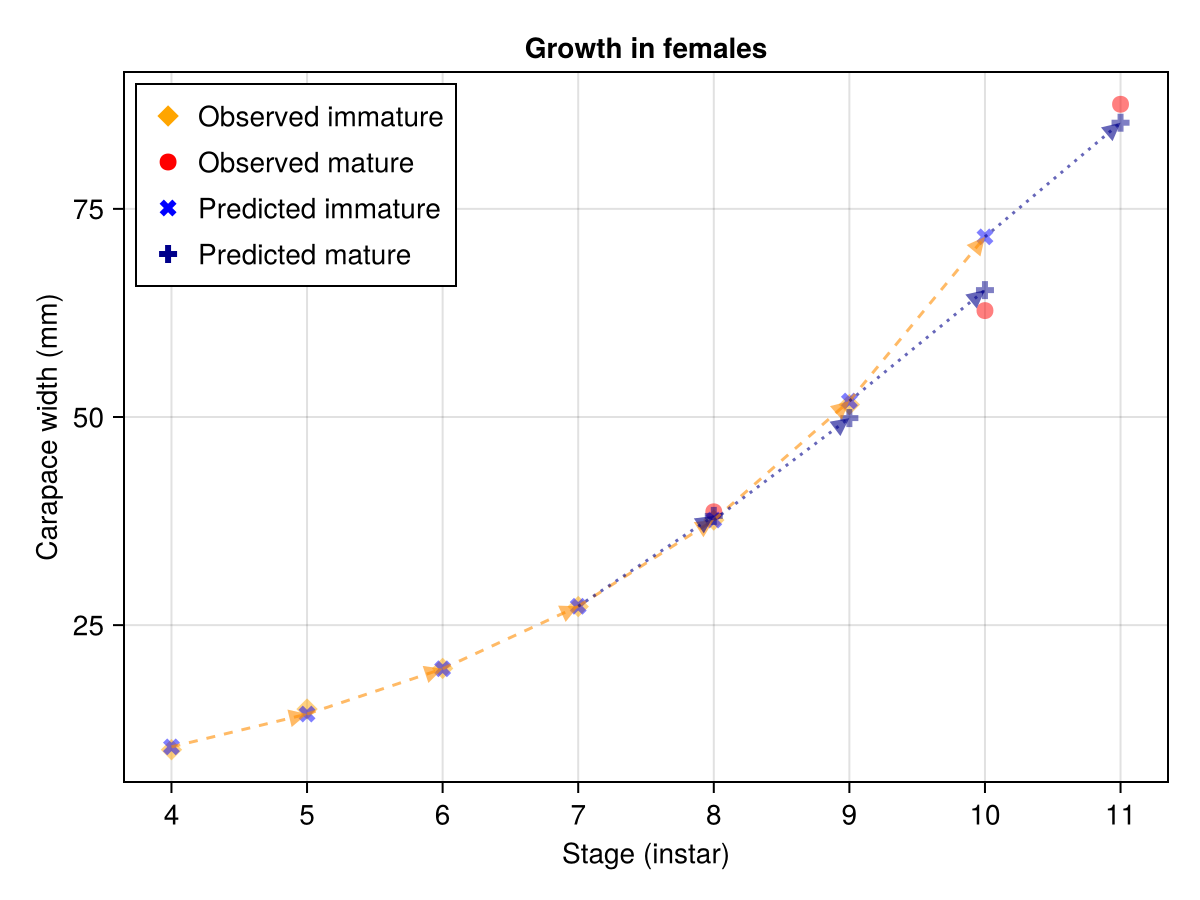
\includegraphics{../../outputs/plot_growth_female.png}
\caption{image}
\end{figure}





 
%% The Appendices part is started with the command \appendix;
%% appendix sections are then done as normal sections
%% \appendix

%% \section{}
%% \label{}

%% References
%%
%% Following citation commands can be used in the body text:
%% Usage of \cite is as follows:
%%   \cite{key}          ==>>  [#]
%%   \cite[chap. 2]{key} ==>>  [#, chap. 2]
%%   \citet{key}         ==>>  Author [#]

%% References with bibTeX database:

 

\printbibliography






%%%%%%%%%%%%%%%%%%%%%%%%%%%%%%%%%%%%%%%%%%%%%%%%%%%%%%%%%%%%
%%% SUPPLEMENTARY MATERIAL / APPENDICES
%%%%%%%%%%%%%%%%%%%%%%%%%%%%%%%%%%%%%%%%%%%%%%%%%%%%%%%%%%%%

% 
%%%%%%%%%%%%%%%%%%%%%%%%%%%%%%%%%%%%%%%%%%%%%%%%%%%%%%%%%%%%
%%% ARTICLE END
%%%%%%%%%%%%%%%%%%%%%%%%%%%%%%%%%%%%%%%%%%%%%%%%%%%%%%%%%%%%

%  

% % \end{CSLReferences}

\end{document}
% \endinput
